% Created 2024-02-21 Wed 22:01
% Intended LaTeX compiler: pdflatex
\documentclass[a4paper,11pt]{exam}
\usepackage[utf8]{inputenc}
\usepackage[T1]{fontenc}
\usepackage{graphicx}
\usepackage{longtable}
\usepackage{wrapfig}
\usepackage{rotating}
\usepackage[normalem]{ulem}
\usepackage{amsmath}
\usepackage{amssymb}
\usepackage{capt-of}
\usepackage{hyperref}
\usepackage[T1]{fontenc}
\usepackage{titling}
\usepackage{url}
\usepackage{amsmath,amsthm,amssymb}
\usepackage{titling}
\usepackage{url}
\usepackage{amsmath,amsthm,amssymb}
\usepackage{graphicx}
\usepackage{graphics}
\usepackage{listings}
\usepackage[dvipsnames]{xcolor}
\usepackage{tabularx}
\usepackage{ragged2e}
\usepackage{courier}
\usepackage{textcomp}
\usepackage{circuitikz}
\usepackage{tikz}
\usepackage{enumitem}
\usepackage{karnaugh-map}
\usepackage{bytefield}
\usepackage{mathrsfs}
\usepackage{cancel}
\usepackage[linesnumbered,ruled,vlined]{algorithm2e}
\usepackage{hyperref}
\usepackage{environ}
\usepackage{listings}
\usepackage{algorithm}
\usepackage{algpseudocode}
\lstset{breaklines=true, basicstyle=\ttfamily\tiny, frame=single, escapeinside={(*@}{@*)}}
\usepackage[margin=0.75in]{geometry}
\author{Miguel Gomez U1318856}
\date{2024-02-21 22:01:27}
\title{Homework Assignment \# 2}
\hypersetup{
 pdfauthor={Miguel Gomez U1318856},
 pdftitle={Homework Assignment \# 2},
 pdfkeywords={},
 pdfsubject={},
 pdfcreator={Emacs 28.2 (Org mode 9.4.6)}, 
 pdflang={English}}
\begin{document}

\maketitle
\tableofcontents

\(\newpage\)
\section{Problem 1}
\label{sec:org05a5948}
\subsection{a)}
\label{sec:org4d37062}
Consider the polynomial $P(x) = x^5 + x^2 + 1 \in \mathbb{F}_2[x]$ with coefficients in the finite field $\mathbb{F}_2$.
You are asked to check if this polynomial is a primitive polynomial. Describe an approach to test if $P(x)$ is primitive. [Refer to the lecture slides on primitive polynomials and LFSRs]. Write a program in Singular to test if $P(x)$ is a primitive polynomial.

\subsubsection{Describing the approach}
\label{sec:org50bd0c6}
Testing whether or not a $P(x)$ is a primitive requires a proof of the properties of the primitive polynomial. To do this, we can show that $P(x) \in \mathbb{F}_2[x]$ has a degree such that the smallest integer $n$ that allows $P(x)$ to divide $x^n + 1$ is $2^k - 1$. So for our case, we would like to show that $n = 2^5 - 1 = 31$. We can do this with the code we wrote in HW 1 for checking the gcd of the target, or just perform the exhaustive calculation showing the gcd being 1 for all except our target. \\\\
Additionally, we could show that the primitive polynomial is capable of generating all exponents? \textcolor{red}{reword this} 

\subsubsection{Program output}
\label{sec:org55dc8f2}
\begin{lstlisting}[language=sing]
                     SINGULAR                                 /  Development
 A Computer Algebra System for Polynomial Computations       /   version 4.3.2
                                                           0<
 by: W. Decker, G.-M. Greuel, G. Pfister, H. Schoenemann     \   Feb 2023
FB Mathematik der Universitaet, D-67653 Kaiserslautern        \
// ** executing /home/speedy/repos/singular/git/Singular/Singular/Singular/.libs/../LIB/.singularrc
degree k = 5
Printing gcd(x5+x2+1, x1 + 1): 1
Printing gcd(x5+x2+1, x2 + 1): 1
Printing gcd(x5+x2+1, x3 + 1): 1
Printing gcd(x5+x2+1, x4 + 1): 1
Printing gcd(x5+x2+1, x5 + 1): 1
Printing gcd(x5+x2+1, x6 + 1): 1
Printing gcd(x5+x2+1, x7 + 1): 1
Printing gcd(x5+x2+1, x8 + 1): 1
Printing gcd(x5+x2+1, x9 + 1): 1
Printing gcd(x5+x2+1, x10 + 1): 1
Printing gcd(x5+x2+1, x11 + 1): 1
Printing gcd(x5+x2+1, x12 + 1): 1
Printing gcd(x5+x2+1, x13 + 1): 1
Printing gcd(x5+x2+1, x14 + 1): 1
Printing gcd(x5+x2+1, x15 + 1): 1
Printing gcd(x5+x2+1, x16 + 1): 1
Printing gcd(x5+x2+1, x17 + 1): 1
Printing gcd(x5+x2+1, x18 + 1): 1
Printing gcd(x5+x2+1, x19 + 1): 1
Printing gcd(x5+x2+1, x20 + 1): 1
Printing gcd(x5+x2+1, x21 + 1): 1
Printing gcd(x5+x2+1, x22 + 1): 1
Printing gcd(x5+x2+1, x23 + 1): 1
Printing gcd(x5+x2+1, x24 + 1): 1
Printing gcd(x5+x2+1, x25 + 1): 1
Printing gcd(x5+x2+1, x26 + 1): 1
Printing gcd(x5+x2+1, x27 + 1): 1
Printing gcd(x5+x2+1, x28 + 1): 1
Printing gcd(x5+x2+1, x29 + 1): 1
Printing gcd(x5+x2+1, x30 + 1): 1
Printing gcd(x5+x2+1, x31 + 1): x5+x2+1
First iteration reached: x^31 + 1
Is Primitive Poly.
Auf Wiedersehen.
Execution Time: .056282630 seconds
\end{lstlisting}

\subsection{b)}
\label{sec:orgcfcdd02}
Design a Type-I or Type-II linear feedback shift register (LFSR) using the above $P(x)$ as its characteristic polynomial. Starting with a non-0 seed value (reset values in the LFSR flip-flops should be non-zero), does your LFSR produce a maximal-length pseudo-random sequence? Show the 5-bit sequences produced by your LFSR. You can do this in Verilog (preferable), or Singular, or any other software.
\newpage

\subsubsection{LFSR Design}
\label{sec:orge378653}
Design of the LFSR uses a DFF module and a 5-bit collection made of 5 DFFs in a row. The bits produce a maximal sequence as can be seen in the verilog output below. There is a copy of the testbench and LFSR.v as well as the DFF.v in the homework files:
\subsubsection{Showing the maximal-length pseudo-random output}
\label{sec:org2774d12}
Below we can see that the LFSR cylces through all combinations of \(2^5\) before repeating, as expected. Here is a block of it running in emacs after compilation

\begin{lstlisting}
-*- mode: compilation; default-directory: "~/repos/courses/hw_crypto/hw2/verilog/testbenches/" -*-
Compilation started at Sun Feb 18 18:02:16

vlog +cover=bcesfx -work /home/speedy/repos/courses/hw_crypto/hw2/verilog/testbenches/work /home/speedy/repos/courses/hw_crypto/hw2/verilog/testbenches/TB_LFSR.v && vsim -c -do "vlib /home/speedy/repos/courses/hw_crypto/hw2/verilog/testbenches/work; vmap work /home/speedy/repos/courses/hw_crypto/hw2/verilog/testbenches/work; vsim work.LFSR_5bit_tb; add wave -r /*; run -all;" 
Model Technology ModelSim - Intel FPGA Edition vlog 2020.1 Compiler 2020.02 Feb 28 2020
Start time: 18:02:16 on Feb 18,2024
vlog "+cover=bcesfx" -work /home/speedy/repos/courses/hw_crypto/hw2/verilog/testbenches/work /home/speedy/repos/courses/hw_crypto/hw2/verilog/testbenches/TB_LFSR.v 
-- Compiling module my_DFF
-- Compiling module LFSR
-- Compiling module LFSR_5bit_tb

Top level modules:
	LFSR_5bit_tb
End time: 18:02:16 on Feb 18,2024, Elapsed time: 0:00:00
Errors: 0, Warnings: 0
Reading pref.tcl

# 2020.1

# vlib /home/speedy/repos/courses/hw_crypto/hw2/verilog/testbenches/work
# ** Warning: (vlib-34) Library already exists at "/home/speedy/repos/courses/hw_crypto/hw2/verilog/testbenches/work".
#  vmap work /home/speedy/repos/courses/hw_crypto/hw2/verilog/testbenches/work
# Model Technology ModelSim - Intel FPGA Edition vmap 2020.1 Lib Mapping Utility 2020.02 Feb 28 2020
# vmap work /home/speedy/repos/courses/hw_crypto/hw2/verilog/testbenches/work 
# Modifying modelsim.ini
#  vsim work.LFSR_5bit_tb
# vsim work.LFSR_5bit_tb 
# Start time: 18:02:16 on Feb 18,2024
# Loading work.LFSR_5bit_tb
# Loading work.LFSR
# Loading work.my_DFF
#  add wave -r /*
#  run -all
# State	Time	Clk	Reset	Q
# 1	0	0	1	00100
# 1	5	1	1	00100
# 1	10	0	0	00100
# 2	15	1	0	01000
# 2	20	0	0	01000
# 3	25	1	0	10000
# 3	30	0	0	10000
# 4	35	1	0	00001
# 4	40	0	0	00001
# 5	45	1	0	00010
# 5	50	0	0	00010
# 6	55	1	0	00101
# 6	60	0	0	00101
# 7	65	1	0	01010
# 7	70	0	0	01010
# 8	75	1	0	10101
# 8	80	0	0	10101
# 9	85	1	0	01011
# 9	90	0	0	01011
# 10	95	1	0	10111
# 10	100	0	0	10111
# 11	105	1	0	01110
# 11	110	0	0	01110
# 12	115	1	0	11101
# 12	120	0	0	11101
# 13	125	1	0	11011
# 13	130	0	0	11011
# 14	135	1	0	10110
# 14	140	0	0	10110
# 15	145	1	0	01100
# 15	150	0	0	01100
# 16	155	1	0	11000
# 16	160	0	0	11000
# 17	165	1	0	10001
# 17	170	0	0	10001
# 18	175	1	0	00011
# 18	180	0	0	00011
# 19	185	1	0	00111
# 19	190	0	0	00111
# 20	195	1	0	01111
# 20	200	0	0	01111
# 21	205	1	0	11111
# 21	210	0	0	11111
# 22	215	1	0	11110
# 22	220	0	0	11110
# 23	225	1	0	11100
# 23	230	0	0	11100
# 24	235	1	0	11001
# 24	240	0	0	11001
# 25	245	1	0	10011
# 25	250	0	0	10011
# 26	255	1	0	00110
# 26	260	0	0	00110
# 27	265	1	0	01101
# 27	270	0	0	01101
# 28	275	1	0	11010
# 28	280	0	0	11010
# 29	285	1	0	10100
# 29	290	0	0	10100
# 30	295	1	0	01001
# 30	300	0	0	01001
# 31	305	1	0	10010
# 31	310	0	0	10010
# 0	315	1	0	00100
# 0	320	0	0	00100
# Success: LFSR returned to initial state 00100 at time               325000
# 1	325	1	0	01000
# 1	330	0	0	01000
# 2	335	1	0	10000
# 2	340	0	0	10000
# 3	345	1	0	00001
# 3	350	0	0	00001
# 4	355	1	0	00010
# 4	360	0	0	00010
# 5	365	1	0	00101
# 5	370	0	0	00101
# 6	375	1	0	01010
# 6	380	0	0	01010
# ** Note: $finish    : /home/speedy/repos/courses/hw_crypto/hw2/verilog/testbenches/TB_LFSR.v(43)
#    Time: 385 ns  Iteration: 1  Instance: /LFSR_5bit_tb
# End time: 18:02:16 on Feb 18,2024, Elapsed time: 0:00:00
# Errors: 0, Warnings: 0

Compilation finished at Sun Feb 18 18:02:17
  \end{lstlisting}

\subsection{c)}
\label{sec:orge4d5bfc}
Refer to Fig. 1. Using a 5-bit plaintext P, and a seed (reset) value for your LFSR, demonstrate that your LFSR can indeed be used as a stream cipher to encrypt (compute C) and decrypt (get back P) one-bit at a time. Once again, it is convenient to demonstrate this using Verilog coding and simulation.
\subsubsection{Stream Cypher Results \(P\Rightarrow{}C\Rightarrow{}P\)}
\label{sec:orgaa4711b}
The results of the system above, working is shown below. This was accomplished using the same LFSR testbench.
\begin{lstlisting}
: Time	P	Q	C	decrypted
: 345	01101	10000	11101	(*@\textcolor{red}{xxxx}@*)1
: 355	01101	00001	01100	(*@\textcolor{red}{xxx}@*)01
: 365	01101	00010	01111	(*@\textcolor{red}{xx}@*)101
: 375	01101	00101	01000	(*@\textcolor{red}{x}@*)1101
: 385	01101	01010	00111	01101
  \end{lstlisting}

\section{Problem 2}
\label{sec:org93f0c14}
Mastrovito Multiplier Design - In this question, you will design a digital logic circuit of a Mastrovito multiplier, i.e. the one that computes A · B (mod P(x)), as given in my slides. You will implement your design in Verilog, and demonstrate – by means of exhaustive simulation – that modulo-multiplication is being performed. Proceed as follows:

\subsection{a)}
\label{sec:org9e5e61a}

We will use the finite field \(\mathbb{F}_8 \equiv \mathbb{F}_2[x] (\text{mod } P(x) = x^3 + x^2 + 1)\) with \(P(\alpha) = 0\). Denote the degree of  \(P(x)\) as \(k\); of course, here \(k = 3\).
\subsection{b)}
\label{sec:org0473801}
Design a \(k = 3\) bit finite field Mastrovito multiplier that takes \(A = \{a2 , a1 , a0\}\) and \(B = \{b2 , b1, b0 \}\) as 3-bit inputs, and produces \(Z = \{z2, z1 , z0 \}\) as a 3-bit output. Note that we will have:
\begin{align*}
A &= a_0 + a_1 \alpha + a_2\alpha^2\\
B &= b_0 + b_1 \alpha + b_2\alpha^2\\
Z &= z_0 + z_1 \alpha + z_2\alpha^2
\end{align*}
Such that \(Z = A \cdot B\pmod{P(\alpha)}\).
\subsection{c)}
\label{sec:org40696b1}
Give Boolean equations (or polynomial equations (mod 2)) of the outputs in terms of inputs, and draw the gate-level schematic. We covered Mastrovito multiplier design in the class when we studied GF circuits. It is given in the slides and in my Book Chapter that I’ve uploaded on Canvas.
\begin{center}
\begin{array}{cccccc}
    & & a_2 & a_1 & a_0 \\
   \times & & b_2 & b_1 & b_0 \\
\cline{1-6}
   & & a_2 \cdot b_0 & a_1 \cdot b_0 & a_0 \cdot b_0 &   \\
   & a_2 \cdot b_1 & a_1 \cdot b_1 & a_0 \cdot b_1 &     \\
   a_2 \cdot b_2 & a_1 \cdot b_2 & a_0 \cdot b_2  &  & \\\cline{1-6}
   s_4 & s_3 & s_2 & s_1 & s_0 \\
\end{array}
\end{center}
\begin{align*}
  s_0 &=  a_0 \cdot b_0 \\
  s_1 &=  a_1 \cdot b_0 + a_0 \cdot b_1 \\
  s_2 &=  a_2 \cdot b_0 + a_1 \cdot b_1 + a_0 \cdot b_2 \\
  s_3 &=  a_2 \cdot b_1 +  a_1 \cdot b_2\\
  s_4 &=  a_2 \cdot b_2
\end{align*}
The result is larger than our bit length so we must perform modulo reduction on the parts that go beyond our length. \(s_3\) and \(s_4\) must be reduced.
  \begin{lstlisting}
printing A^0 = 1
printing A^1 = (A)
printing A^2 = (A2)
printing A^3 = (A2+1)
printing A^4 = (A2+A+1)
printing A^5 = (A+1)
printing A^6 = (A2+A)
printing A^7 = 1
Auf Wiedersehen.  
  \end{lstlisting}

Given the reduction we can see above, we will be replacing \(\alpha^3\) and \(\alpha^4\) with \(\alpha^2+1\) and \(\alpha^2 + \alpha + 1\) respectively. 

\begin{align*}
  \alpha^3 &= \alpha^2 + 1\\
  \alpha^4 &= \alpha^2 + \alpha + 1
\end{align*}
\begin{align*}
  S &= s_0 + s_1 \alpha + s_2 \alpha^2 + s_3 \alpha^3 + s_4 \alpha^4 \\
  S &= s_0 + s_1 \alpha + s_2 \alpha^2 + s_3 (\alpha^2 + 1) + s_4 (\alpha^2 + \alpha + 1)  \\
  S &= (s_0 + s_3 + s_4) + (s_1 + s_4)\alpha + (s_2 + s_3 + s_4)\alpha^2
\end{align*}
\begin{align*}
Z_0 &= S_0 = s_0 + s_3 + s_4\\
Z_1 &= S_1 = s_1 + s_4\\
Z_2 &= S_2 = s_2 + s_3 + s_4\\
\end{align*}



\subsection{d)}
\label{sec:orgf6ad2a8}
Implement the design in Verilog (as a GFMult(A, B, Z) module) and demonstrate its correctness via exhaustive simulation.
\begin{lstlisting}
Time	A	B	Z
0	000	000	xxx
0	000	000	000
25	001	000	000
75	010	000	000
125	011	000	000
175	100	000	000
225	101	000	000
275	110	000	000
325	111	000	000
375	000	001	000
425	001	001	000
450	001	001	001
475	010	001	001
500	010	001	010
525	011	001	010
550	011	001	011
575	100	001	011
600	100	001	100
625	101	001	100
650	101	001	101
675	110	001	101
700	110	001	110
725	111	001	110
750	111	001	111
775	000	010	111
800	000	010	000
825	001	010	000
850	001	010	010
875	010	010	010
900	010	010	100
925	011	010	100
950	011	010	110
975	100	010	110
1000	100	010	101
1025	101	010	101
1050	101	010	111
1075	110	010	111
1100	110	010	001
1125	111	010	001
1150	111	010	011
1175	000	011	011
1200	000	011	000
1225	001	011	000
1250	001	011	011
1275	010	011	011
1300	010	011	110
1325	011	011	110
1350	011	011	101
1375	100	011	101
1400	100	011	001
1425	101	011	001
1450	101	011	010
1475	110	011	010
1500	110	011	111
1525	111	011	111
1550	111	011	100
1575	000	100	100
1600	000	100	000
1625	001	100	000
1650	001	100	100
1675	010	100	100
1700	010	100	101
1725	011	100	101
1750	011	100	001
1775	100	100	001
1800	100	100	111
1825	101	100	111
1850	101	100	011
1875	110	100	011
1900	110	100	010
1925	111	100	010
1950	111	100	110
1975	000	101	110
2000	000	101	000
2025	001	101	000
2050	001	101	101
2075	010	101	101
2100	010	101	111
2125	011	101	111
2150	011	101	010
2175	100	101	010
2200	100	101	011
2225	101	101	011
2250	101	101	110
2275	110	101	110
2300	110	101	100
2325	111	101	100
2350	111	101	001
2375	000	110	001
2400	000	110	000
2425	001	110	000
2450	001	110	110
2475	010	110	110
2500	010	110	001
2525	011	110	001
2550	011	110	111
2575	100	110	111
2600	100	110	010
2625	101	110	010
2650	101	110	100
2675	110	110	100
2700	110	110	011
2725	111	110	011
2750	111	110	101
2775	000	111	101
2800	000	111	000
2825	001	111	000
2850	001	111	111
2875	010	111	111
2900	010	111	011
2925	011	111	011
2950	011	111	100
2975	100	111	100
3000	100	111	110
3025	101	111	110
3050	101	111	001
3075	110	111	001
3100	110	111	101
3125	111	111	101
3150	111	111	010
\end{lstlisting}

Above we can see the exhaustive printed results of the multiplier. As an example, the final row we see gives
\begin{center}
 \begin{array}{cccc}
time & A & B & Z\\
3150 & 111 & 111 & 010
\end{array} 
\end{center}
This corresponds ot the following:
\begin{align*}
  111 \cdot 111 &= 010 \\
  (\alpha^2 + \alpha + 1)\cdot(\alpha^2 + \alpha + 1) &= \alpha
\end{align*}
The expression above can be shown to reduce to $\alpha$ by replacing $\alpha^3$ with $\alpha^2 + 1$, and $\alpha^4$ with $\alpha^2 + \alpha + 1$-the rest will reduce in a similar way giving us the expected results.
\begin{align*}
  (\alpha^2 + \alpha + 1)\cdot(\alpha^2 + \alpha + 1) &= \alpha\\
  (\alpha^2 + \alpha + 1)\cdot\alpha^2 + (\alpha^2 + \alpha + 1)\cdot\alpha + (\alpha^2 + \alpha + 1) &= \\
  (\alpha^4 + \alpha^3 + \alpha^2)  + (\alpha^3 + \alpha^2 + \alpha) + (\alpha^2 + \alpha + 1) &= \\
  \alpha^4 + 2\alpha^3 + 3\alpha^2 + 2\alpha + 1 &= \\
  \alpha^4 + \textcolor{red}{\cancelto{\textcolor{black}{0}}{\textcolor{black}{2\alpha^3}}} + 3\alpha^2 + \textcolor{red}{\cancelto{\textcolor{black}{0}}{\textcolor{black}{2\alpha}}} + 1 &= \\
  \alpha^4 + 3\alpha^2  + 1 &=  \alpha^2 + \alpha + 1 + 3\alpha^2  + 1\\
                                                      &=  \textcolor{red}{\cancelto{\textcolor{black}{0}}{\textcolor{black}{4\alpha^2}}} + \alpha   + \textcolor{red}{\cancelto{\textcolor{black}{0}}{\textcolor{black}{2}}}\\
                                                      &= \alpha
\end{align*}


\subsection{e)}
\label{sec:org4337674}
Using any Verilog synthesis and simulation tool, synthesize the circuit into a netlist.
\begin{figure}[h]
\centering
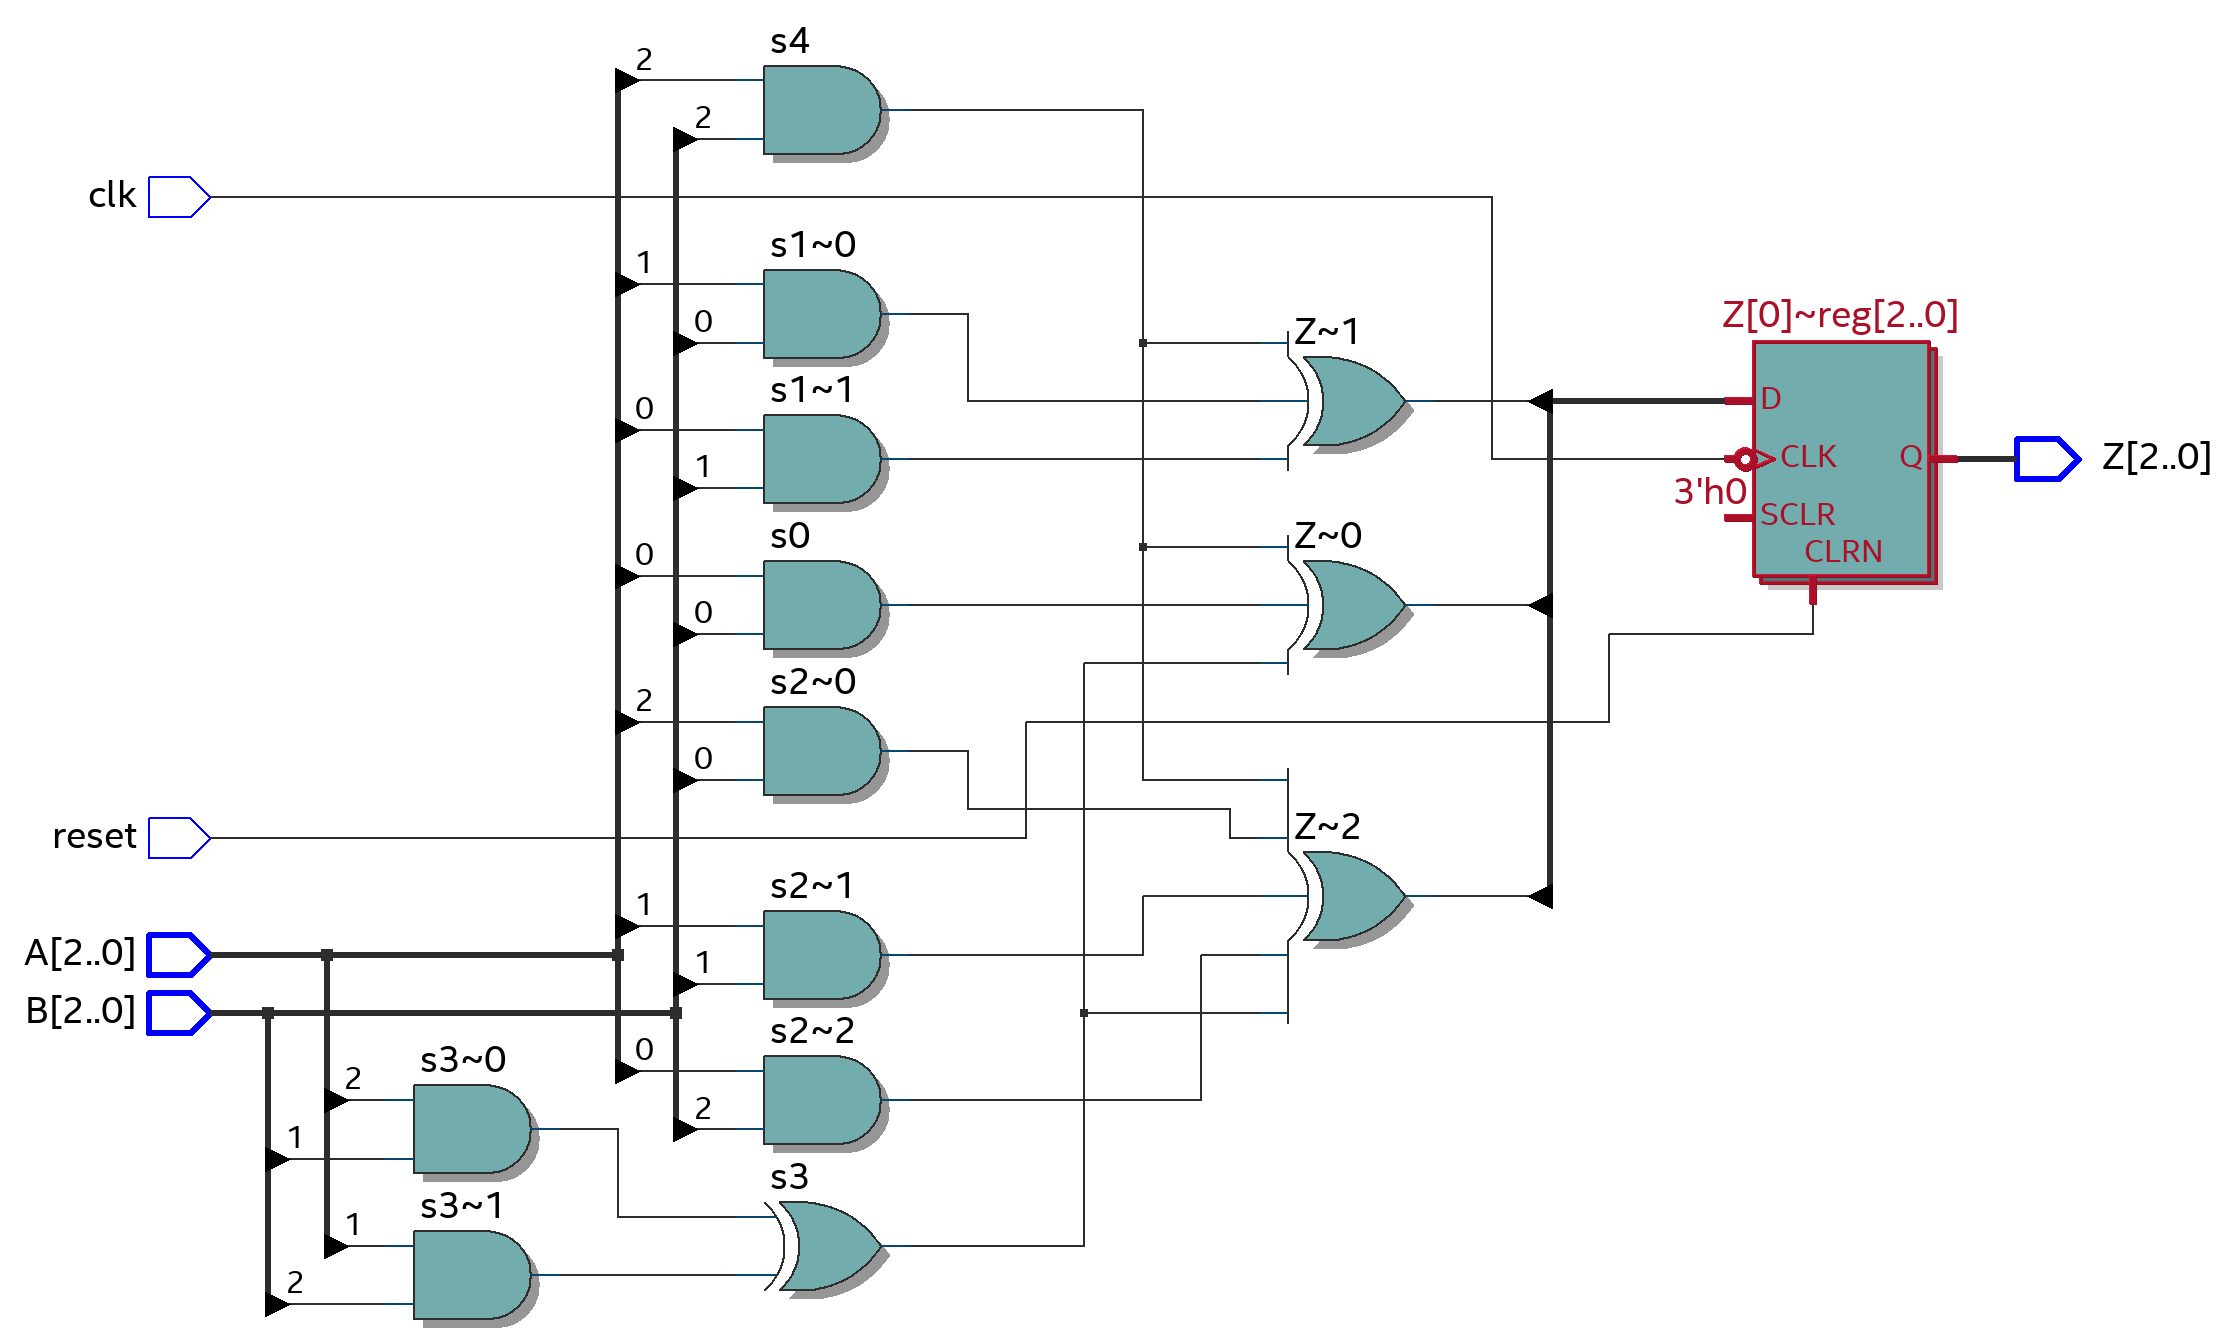
\includegraphics[width=10cm]{./images/TechnologyMap_GFMult.png}
  \caption{multiplier netlist view}
  \label{fig:gfmult}
\end{figure}  

\subsection{f)}
\label{sec:org85464cf}
Using any of the Cyclone V devices, synthesize the circuit for the selected FPGA architecture.
\begin{itemize}
\item Done.
\end{itemize}

\subsection{g)}
\label{sec:orgee04339}
Note down the area and the delay of the circuit. The synthesis tools will give this information in the synthesis report. Area could be the actual area, or in terms of the number of gates, or in terms of the number of LUTs of the FPGA. Delay could be the actual delay, or the topological depth of the circuit.
\begin{itemize}
\item Bit fuzzy on where this data is. \textcolor{red}{REVIEW THIS AND UPDATE BEFORE TURNIN}
\end{itemize}

\section{Problem 3}
\label{sec:org495dea8}
Now you will design a Montgomery multiplier for the same finite field as given above: \\

\begin{center}
$\mathbb{F}_8 \equiv \mathbb{F}_2 [x] (mod P(x) = x^3 + x^2 + 1)$ with $P(\alpha) = 0$.
\end{center}
\subsection{a)}
\label{sec:org2369f9c}
First, you will design a Montgomery Block \(MM(A, B, \alpha^{-k} ) = A \cdot B \cdot \alpha^{-k} (mod P(\alpha))\), as shown in the slides as well as in my book chapter.
\begin{lstlisting}
module MM (
	   input wire [2:0] A,
	   input wire [2:0] B,
	   input wire	   clk,
	   input wire	   reset,
	   output reg [2:0] Z
	   );

   // add in the signals that are combinational below for MM block.

   // this represents the P(x) or 1*x^3 + 1*x^2 + 0*x + 1*1 = 4'b1101
   // a^-k = a^-3 or the cube of the inverse of a, or the inverse of the cube of a.
   // inv of cube is a^4 = a*(a^3) = a*(a^2 + 1) = a^3 + a = a^2 + a + 1 = 0111
   wire [3:0]		    _P = 4'b1101;
   reg [3:0]		    mid0_0;
   reg [3:0]		    mid0_1;
   reg [3:0]		    mid0_2;

   reg [3:0]		    mid1_0;
   reg [3:0]		    mid1_1;
   reg [3:0]		    mid1_2;

   reg [3:0]		    mid2_0;
   reg [3:0]		    mid2_1;
   reg [3:0]		    mid2_2;
   

   
   // previously clocked on posedge reset and negedge clk
   always@(*) begin
      if(reset) begin
	 Z = 3'b0;
      end
      else begin
	 mid0_0 = 4'b0^({4{A[0]}}&B);
	 mid0_1 = mid0_0^({4{mid0_0[0]}}&_P);
	 mid0_2 = mid0_1 >> 1'b1;


	 mid1_0 = mid0_2[1]^({4{A[1]}}&B);
	 mid1_1 = mid1_0^({4{mid1_0[0]}}&_P);
	 mid1_2 = mid1_1 >> 1'b1;


	 mid2_0 = mid1_2[2]^({4{A[2]}}&B);
	 mid2_1 = mid2_0^({4{mid2_0[0]}}&_P);
	 mid2_2 = mid2_1 >> 1'b1;
 	 
	 Z = mid2_2[2:0];      
      // Z[1] <= Z[1]^({A[1],A[1],A[1]}&B);      
      // Z[2] <= Z[2]^({A[2],A[2],A[2]}&B);
      end
   end
endmodule // MM
Execution Time: .002747122 seconds
\end{lstlisting}

\subsection{b)}
\label{sec:org100dffc}
Then, you will put 4 of these blocks together to design a multiplication circuit that computes \(G = A \cdot B (mod P(x))\).

\subsection{c)}
\label{sec:org505573c}
For the design of a MM block, you should use Algorithm 1 in my textbook chapter, unroll the loop k-times and design a \(\text{\it{combinational circuit}}\).
Attempt was made to do this but I am unable to get results that make sense in the overall behavior. Here is a block showing what I came up with:
\begin{lstlisting}
`timescale 1ns / 1ps
`include "../MM.v"
module TB_MM;

   reg        clk;
   reg	      clk2;
   reg	      reset;
   reg [2:0]  A;
   reg [2:0]  B;
   wire [2:0] Z0;
   wire [2:0] Z1;
   wire [2:0] Z2;
   wire [2:0] Z3;
   // P is the poly x^3 + x^2 + 1
   reg [2:0]  P = 3'b111;
   // P_inv is the poly 1 + x^-1 + x^-3
   reg [2:0]  P_inv = 3'b011;
   

   MM uut0 (.A(P),.B(A),.clk(clk),.reset(reset),.Z(Z0));
   MM uut1 (.A(P),.B(B),.clk(clk),.reset(reset),.Z(Z1));
   MM uut2 (.A(Z0),.B(Z1),.clk(clk),.reset(reset),.Z(Z2));
   MM uut3 (.A(Z2),.B(3'b001),.clk(clk),.reset(reset),.Z(Z3));


     // Clock generation
initial begin
    clk = 0;
    forever #5 clk = ~clk; // Generate a clock with a period of 10ns
end

     // Clock generation
initial begin
    clk2 = 0;
    forever #20 clk2 = ~clk2; // Generate a clock with a period of 10ns
end

   always@(posedge clk2) begin
      A = A + 1;
      if(A == 0) begin
	 B = B + 1;
      end
   end

// Test sequence
initial begin
   // Initialize simulation
   //file = $fopen("TB_MM.log", "w");
   //file2 = $fopen("MM_results.log", "w");
   $display("Time\tClk\tA\tB\tZ0\tZ1\tZ2\tZ3");
   //$fwrite(file,"\tTime\tClk\tA\tB\tZ\n");
   $monitor("%g\t%g\t%b\t%b\t%b\t%b\t%b\t%b", $time, clk, A, B, Z0, Z1, Z2, Z3);
   // Reset sequence
   reset = 1; // Activate reset
   #25;       // Hold reset for 10ns
   A = 3'b0;
   B = 3'b0;
   reset = 0; // Deactivate reset to start the LFSR
   

    // Let the LFSR run for a while
    #16500;

    // End simulation
   $display("End of simulation @ %g ns", $time);
   //$fwrite(file,"End of simulation @ %g ns", $time);
   $finish;
   
end // initial begin

   
endmodule
Execution Time: .001868000 seconds
\end{lstlisting}

\subsection{d)}
\label{sec:org2ef8f2a}
 Design the circuit in Verilog.\newline\newline
Done as shown above. Unfortunately it is not working as I was hoping. 
\subsection{e)}
\label{sec:org2d04b26}
Simulate the multiplier exhaustively to demonstrate its correct operation.\newline\newline
Also done in the testbench logic. You can see that I increment A and B through all possible combinations in it before exiting. I would make a comparison to the known results and what it should come out to, but I lost time by focusing on getting the system outputting results as I believed it should. 
\subsection{f)}
\label{sec:orgf0fafa7}
Synthesize the circuit, report the area and delay statistics, comparing it with the Mastrovito
design.\newline\newline
For this, I also lost the ability to get this done since I am unable to get the design working as it should. I can export to the RTL design and compare, but it would be moot if it does not function as intended. The correct design may be much larger or smaller than this, so I cannot produce these results with any level of certainty. 

\section{Problem 4}
\label{sec:org1e42899}
If \(P\) is a primitive polynomial, then \(P^*\) will be as well. Therefore if \(\alpha\) is a root of \(P\), \(\alpha^{-1}\) will be a root of \(P^*\).
\subsection{Showing the process}
\label{sec:orga90ddb8}
\begin{align*}
  P(\alpha) &= 0 \\
  P(x) &= a_0x^{k} +  a_1x^{k-1} + a_2x^{k-2} + \ldots + a_{k-1}x + a_k\\
  P^*\left(\frac{1}{x}\right) &= b_0x^{k} +  b_1x^{k-1} + b_2x^{k-2} + \ldots + b_{k-1}x + b_k\\
  P^*\left(\frac{1}{x}\right) &= b_0\frac{1}{x}^{k} +  b_1\frac{1}{x}^{k-1} + b_2\frac{1}{x}^{k-2} + \ldots + b_{k-1}\frac{1}{x} + b_k \\
  &= b_0x^{-k} +  b_1x^{-k+1} + b_2x^{-k+2} + \ldots + b_{k-1}x^{-1} + b_k
  \end{align*}
  normalizing the expression by $x^k$ should not change the overall expression since $x^k = 1$ by the cyclic nature of the root.
  \begin{align*}
    &= x^k\cdot(b_0x^{-k} +  b_1x^{-k+1} + b_2x^{-k+2} + \ldots + b_{k-1}x^{-1} + b_k)\\
    &= b_0 +  b_1x + b_2x^{2} + \ldots + b_{k-1}x^{k-1} + b_kx^k 
  \end{align*}
  Now we can see that the expression is equal to the first with the coefficients reversed, so there is a symmetry between the $\alpha$ and$\alpha^{-1}$. To give a rigorous proof of this fact requires more than what we have gone over in class, but I believe this should do for now. 
\end{document}